% fancytikzposter.tex, version 2.1
% Original template created by Elena Botoeva [botoeva@inf.unibz.it], June 2012
% 
% This file is distributed under the Creative Commons Attribution-NonCommercial 2.0
% Generic (CC BY-NC 2.0) license
% http://creativecommons.org/licenses/by-nc/2.0/ 


\documentclass{a0poster}

\usepackage{fancytikzposter} 


%%%%% --------- Change here if you want ---------- %%%%%
%% margin for the geometry package, must be changed before using the geometry package
%% default value is 4cm
% \setmargin{4}

%% the space between the blocks
%% default value is 2cm
% \setblockspacing{2}

%% the height of the title stripe in block nodes, decrease it to save space
%% default value is 3cm
% \setblocktitleheight{3}

%% the number of columns in the poster, possible values 2,3
%% default value is 2
% \setcolumnnumber{3}

%% the space between two or more groups of authors from different institutions
%% used in \maketitle
% \setinstituteshift{10}

%% which template to use
%% N1 simple, standard look, with a colored background and gray boxes
%% N2 board with nodes
%% N3 another standard look
%% N4 envelope-like look
%% N5 with a wave-like head, original idea taken from
%%%% http://fc09.deviantart.net/fs71/f/2010/322/1/1/scientific_poster_by_nabuy-d333ria.jpg
\usetemplate{5}

%% components of the templates
%% (the maximal possible numbers are mentioned as the parameters)
% \usecolortemplate{4}
% \usebackgroundtemplate{5}
% \usetitletemplate{2}
% \useblocknodetemplate{5}
% \useplainblocktemplate{4}
% \useinnerblocktemplate{2}


%% the height of the head drawing on top 
%% applicable to templates N3, 4 and 5
% \setheaddrawingheight{14}


%% change the basic colors
%\definecolor{myblue}{HTML}{008888} 
%\setfirstcolor{myblue}% default 116699
%\setsecondcolor{gray!80!}% default CCCCCC
%\setthirdcolor{red!80!black}% default 991111

%% change the more specific colors
% \setbackgrounddarkcolor{colorone!70!black}
% \setbackgroundlightcolor{colorone!70!}
% \settitletextcolor{textcolor}
% \settitlefillcolor{white}
% \settitledrawcolor{colortwo}
% \setblocktextcolor{textcolor}
% \setblockfillcolor{white}
% \setblocktitletextcolor{colorone}
% \setblocktitlefillcolor{colortwo} %the color of the border
% \setplainblocktextcolor{textcolor}
% \setplainblockfillcolor{colorthree!40!}
% \setplainblocktitletextcolor{textcolor}
% \setplainblocktitlefillcolor{colorthree!60!}
% \setinnerblocktextcolor{textcolor}
% \setinnerblockfillcolor{white}
% \setinnerblocktitletextcolor{white}
% \setinnerblocktitlefillcolor{colorthree}




%%% size of the document and the margins
%% A0
% \usepackage[margin=\margin cm, paperwidth=118.9cm, paperheight=84.1cm]{geometry} 
\usepackage[margin=\margin cm, paperwidth=84.1cm, paperheight=118.9cm]{geometry}
%% B1
% \usepackage[margin=\margin cm, paperwidth=70cm, paperheight=100cm]{geometry}



%% changing the fonts
\usepackage{cmbright}
%\usepackage[default]{cantarell}
%\usepackage{avant}
%\usepackage[math]{iwona}
\usepackage[math]{kurier}
\usepackage[T1]{fontenc}
\usepackage{subfig}
\usepackage{graphicx}
\usepackage{float}
%% add your packages here
\usepackage{hyperref}
\usepackage{pifont}
\usepackage[export]{adjustbox}

\def\Put(#1,#2)#3{\leavevmode\makebox(0,0){\put(#1,#2){#3}}}



\title{SIFT descriptor to set landmark on biological images}
\author{Van Linh LE$^{1,3}$, Marie BEURTON-AIMAR$^1$, Adrien KRAHENBUHL$^1$, Nicolas PARISEY$^2$\\
  $^1$LaBRI - UMR 5800, Univ. Bordeaux, $^2$INRA - IGEPP UMR 1349, France $^3$ IT - DLU,Vietnam\\
  \texttt{van-linh.le,beurton,adrien.krahenbuhl@labri.fr,nparisey@rennes.inra.fr}
}


\begin{document}
%%%%% ---------- the background picture ---------- %%%%%
%% to change it modify the macro \BackgroundPicture
\ClearShipoutPicture
\AddToShipoutPicture{\BackgroundPicture}

\noindent % to have the picture right in the center
\begin{tikzpicture}
\Put(-17,80){
\includegraphics[scale=1.8]{images/labri}}
\Put(-9,80){
\includegraphics[scale=1.8]{images/ubordeaux}}
\Put(6,80){
\includegraphics[scale=1.8]{images/inra}}
  \initializesizeandshifts
  % \setxshift{15}
  % \setyshift{2}


  %% the title block, #1 - shift, the default value is (0,0), #2 - width, #3 - scale
  %% the alias of the title block is `title', so we can refer to its boundaries later
  \ifthenelse{\equal{\template}{1}}{ 
    \titleblock{47}{1}
  }{
    \titleblock{47}{1.4}
  }

  %% a logo can be added to the title block
  %% #1 - anchor relative to the title block, #2 - shift, #3 - width, #3 - file name
  % \ifthenelse{\equal{\template}{2}}{ 
  %   \addlogo[south west]{(2,0)}{6cm}{images/color.png}
  % }{
  %   \addlogo[south west]{(2,0)}{6cm}{images/color.png}
  % }


  %% a block node, with the specified position (optional), title and the content
  %% #1 - where (optional), #2 - title, #3 - text
  %%%%%%%%%% ------------------------------------------ %%%%%%%%%%
  \blocknode%
  {Context}%
  {
	  \begin{itemize}
   		 \item \textcolor{colorthree}{\textbf{Morphometry}} analysis is a way to characterize the shape variations of the organisms,
   		 \item Morphometric characteristics have been used to evaluate the evolution of an organism, by finding new or sharpening definition of old one,
   		 \item \textcolor{colorthree}{\textbf{Morphometrics}} are also used to \textcolor{colorthree}{\textbf{classify}} the objects in different groups.
    	  \end{itemize}
%    	  \begin{tikzfigure}
%    	  	\centering
%    	  	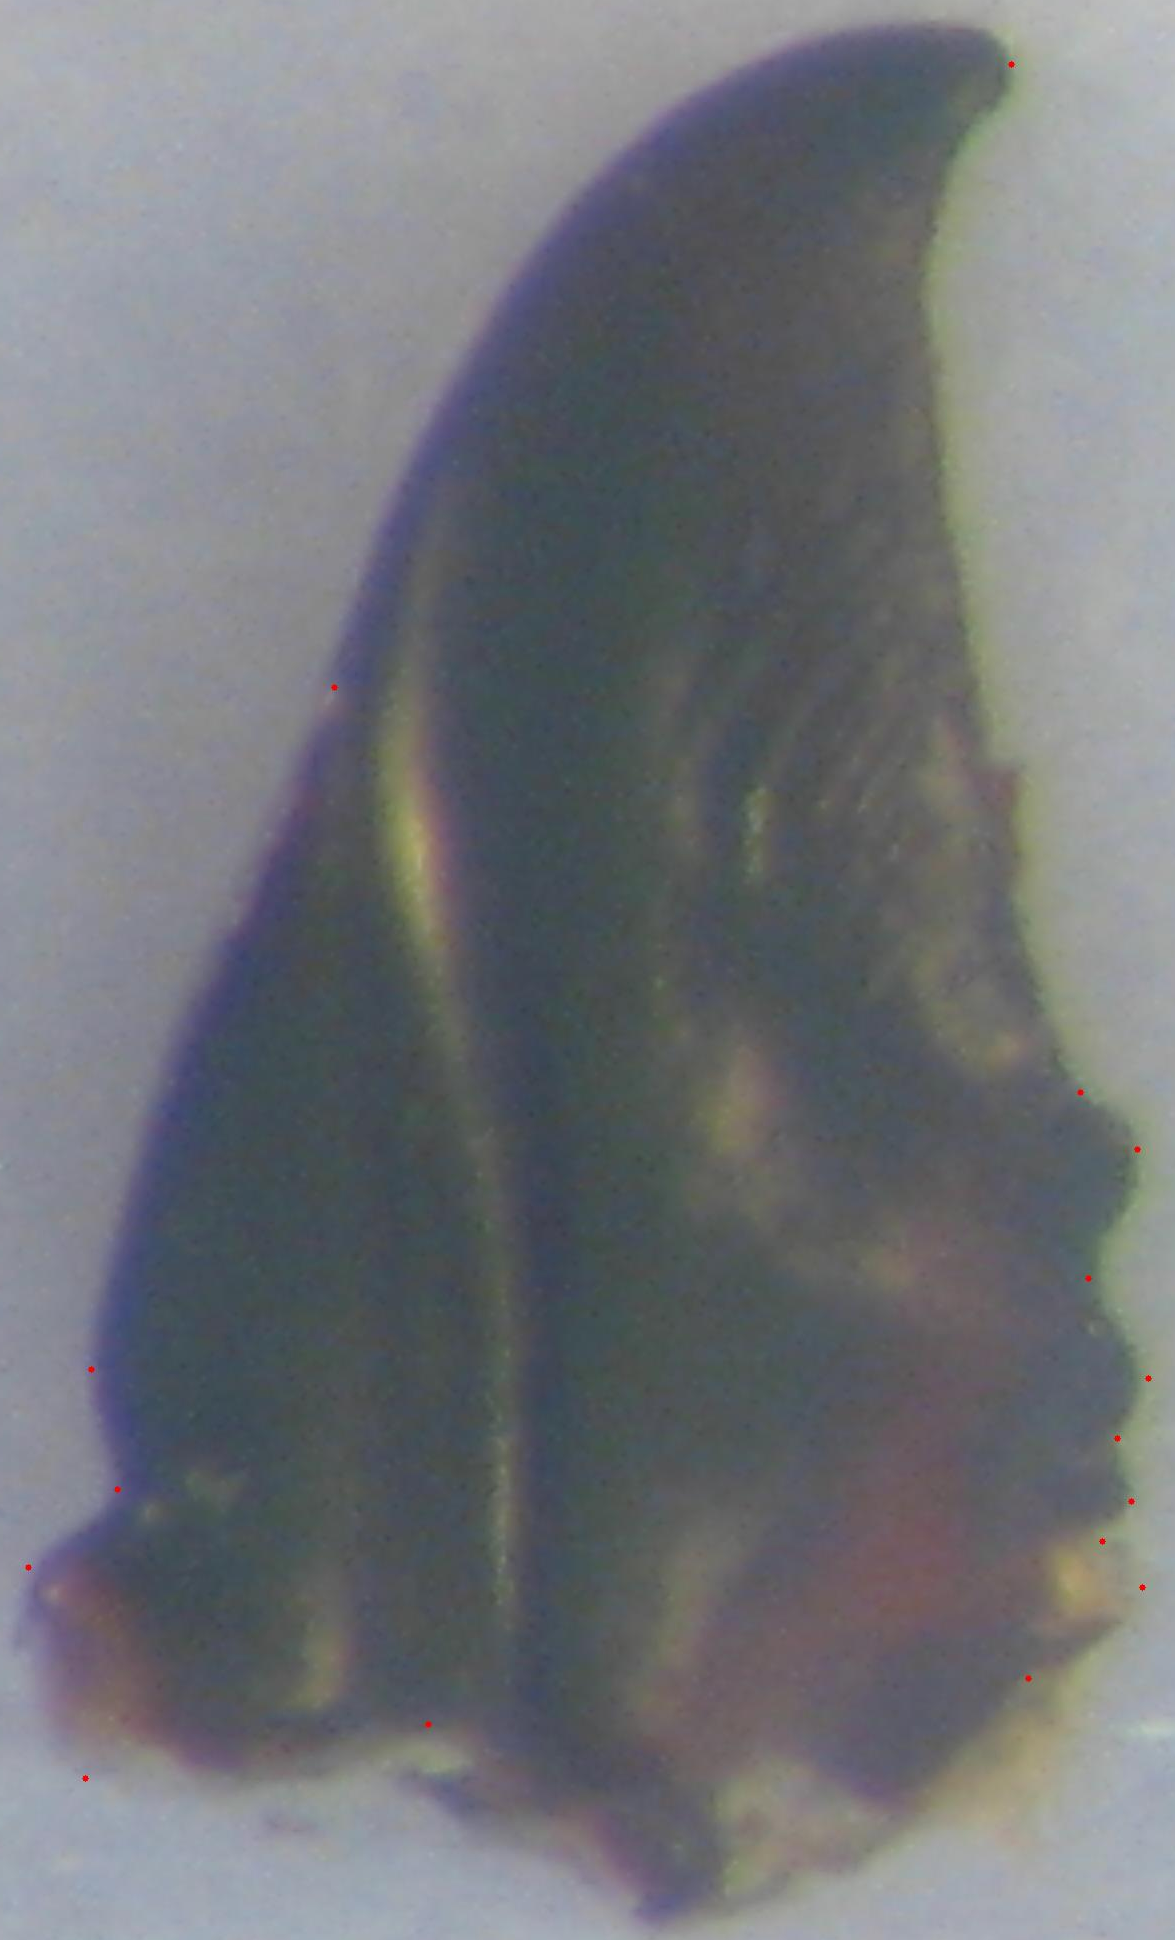
\includegraphics[width=0.3\textwidth]{images/color}~~~~~~
%    	  	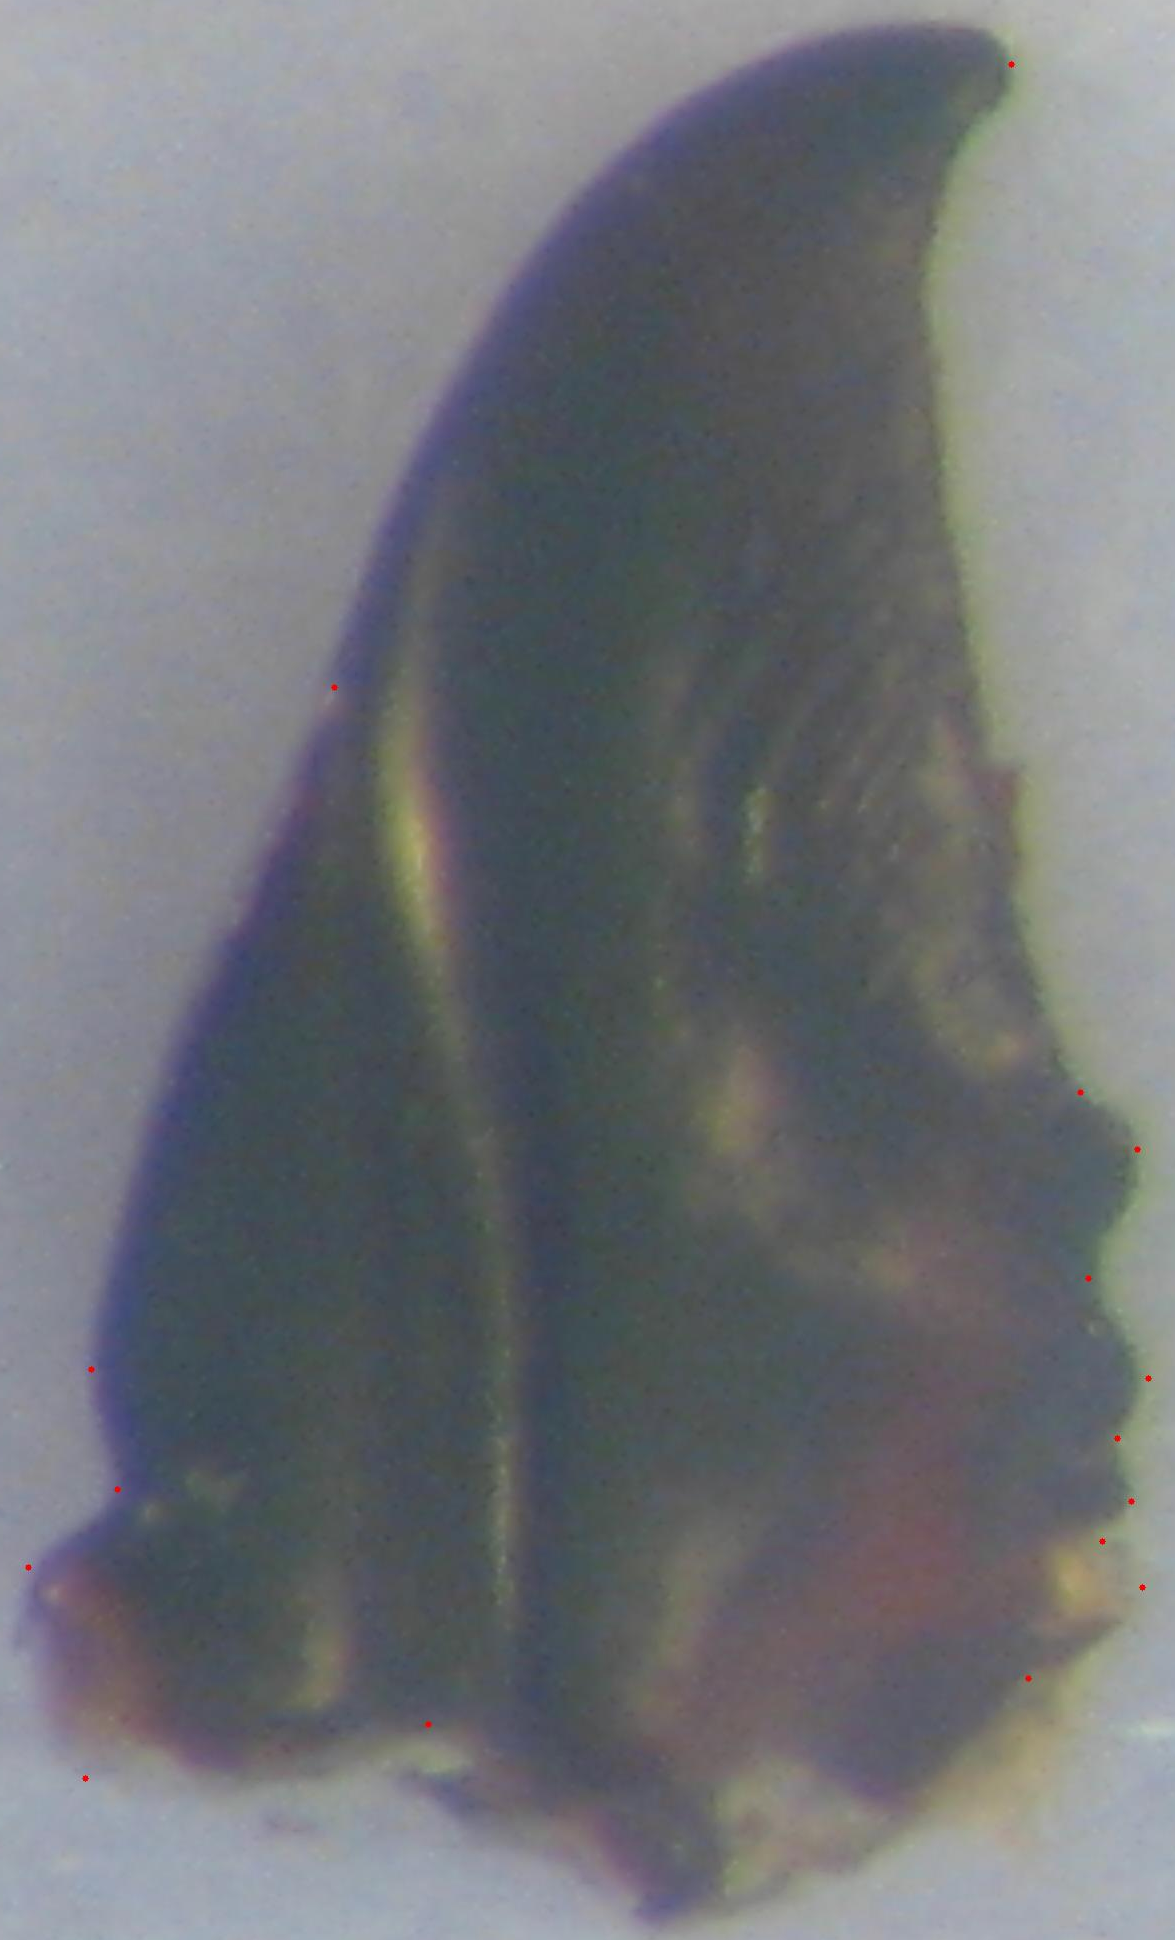
\includegraphics[width=0.3\textwidth]{images/color}
%    	  \end{tikzfigure}
    	  
  }


  %% a callout block
  %% #1 - rotate angle (optional), #2 - from, #3 - where, #4 - width, #5 - text
  %%%%%%%%%% ------------------------------------------ %%%%%%%%%%
  %\calloutblock{($(box.center)+(-2,-8)$)}
  %{($(box.center)+(10,-1)$)}
  %{19cm}
  %{\small
  %  Macro for creating a block node:
  %  \begin{itemize}
  %  \item[] \textbackslash blocknode\{Block Title\}\{Block Content\}
  %  \end{itemize}
  %  Macro \textbackslash blocknode has three parameters. The first one is
  %  optional and it is the position of the block. The first block will be
  %  automatically placed to (\$(firstrow)-(xshift)-(yshift)\$), which is the
  %  left corner below the title block. In most of the templates, (firstrow) is
  %  set to (title.south), where \emph{title} is the alias for the title
  %  block. Each subsequent block is automatically placed to
  %  [(\$(box.south)-(yshift)\$)], i.e., below the previous block aliased
  %  \emph{box}.  You can also use an explicit parameter, e.g., $(-10,30)$ (note
  %  that (0,0) is the center of the poster). The second parameter is the title
  %  of the block. Finally, the last parameter is the  actual content. 
  %}




  %% by default, the position of the new block node is right below the previous
  %% block node, stored in (currenty)
  %% box is the alias of the previous block, so we can refer to its boundaries

  %%%%%%%%%% ------------------------------------------ %%%%%%%%%%
  \blocknode{Manual landmarks}%
  {
  	\begin{itemize}
  		\item Morphometric landmarks are points of interest in biological object,
  		\item Landmarks characterize specificities through the shape \\ most often linked to biological information,
  		\item They are usually \textcolor{colorthree}{\textbf{defined}} by biologists \textcolor{colorthree}{\textbf{manually}},
  		\item Images show manual landmarks in \textcolor{colorthree}{\textbf{beetle mandibles}} \\ belonging to our sample. 
  		
  	\end{itemize}
  	\Put(23,7){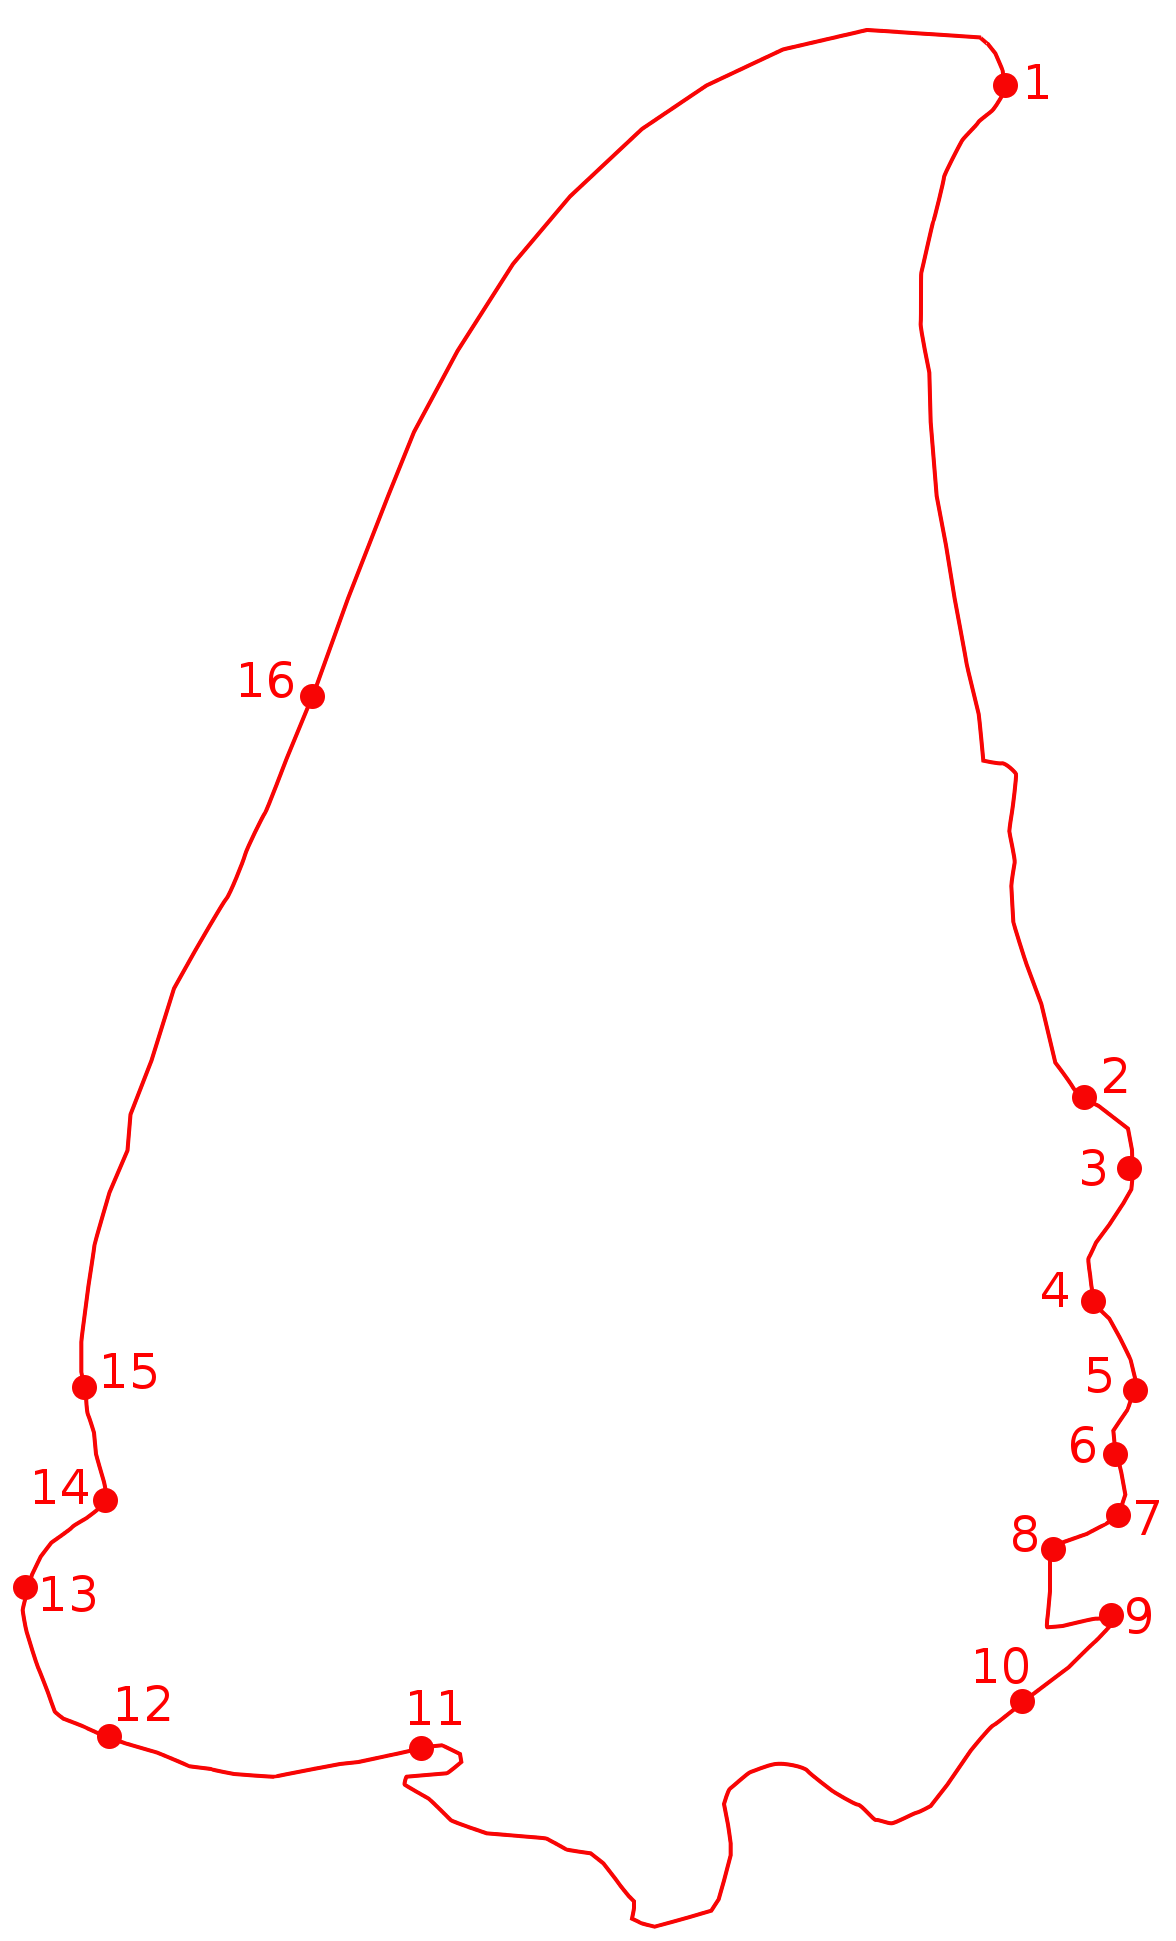
\includegraphics[scale=.3]{images/mlandmarksline}}
    \Put(29,7){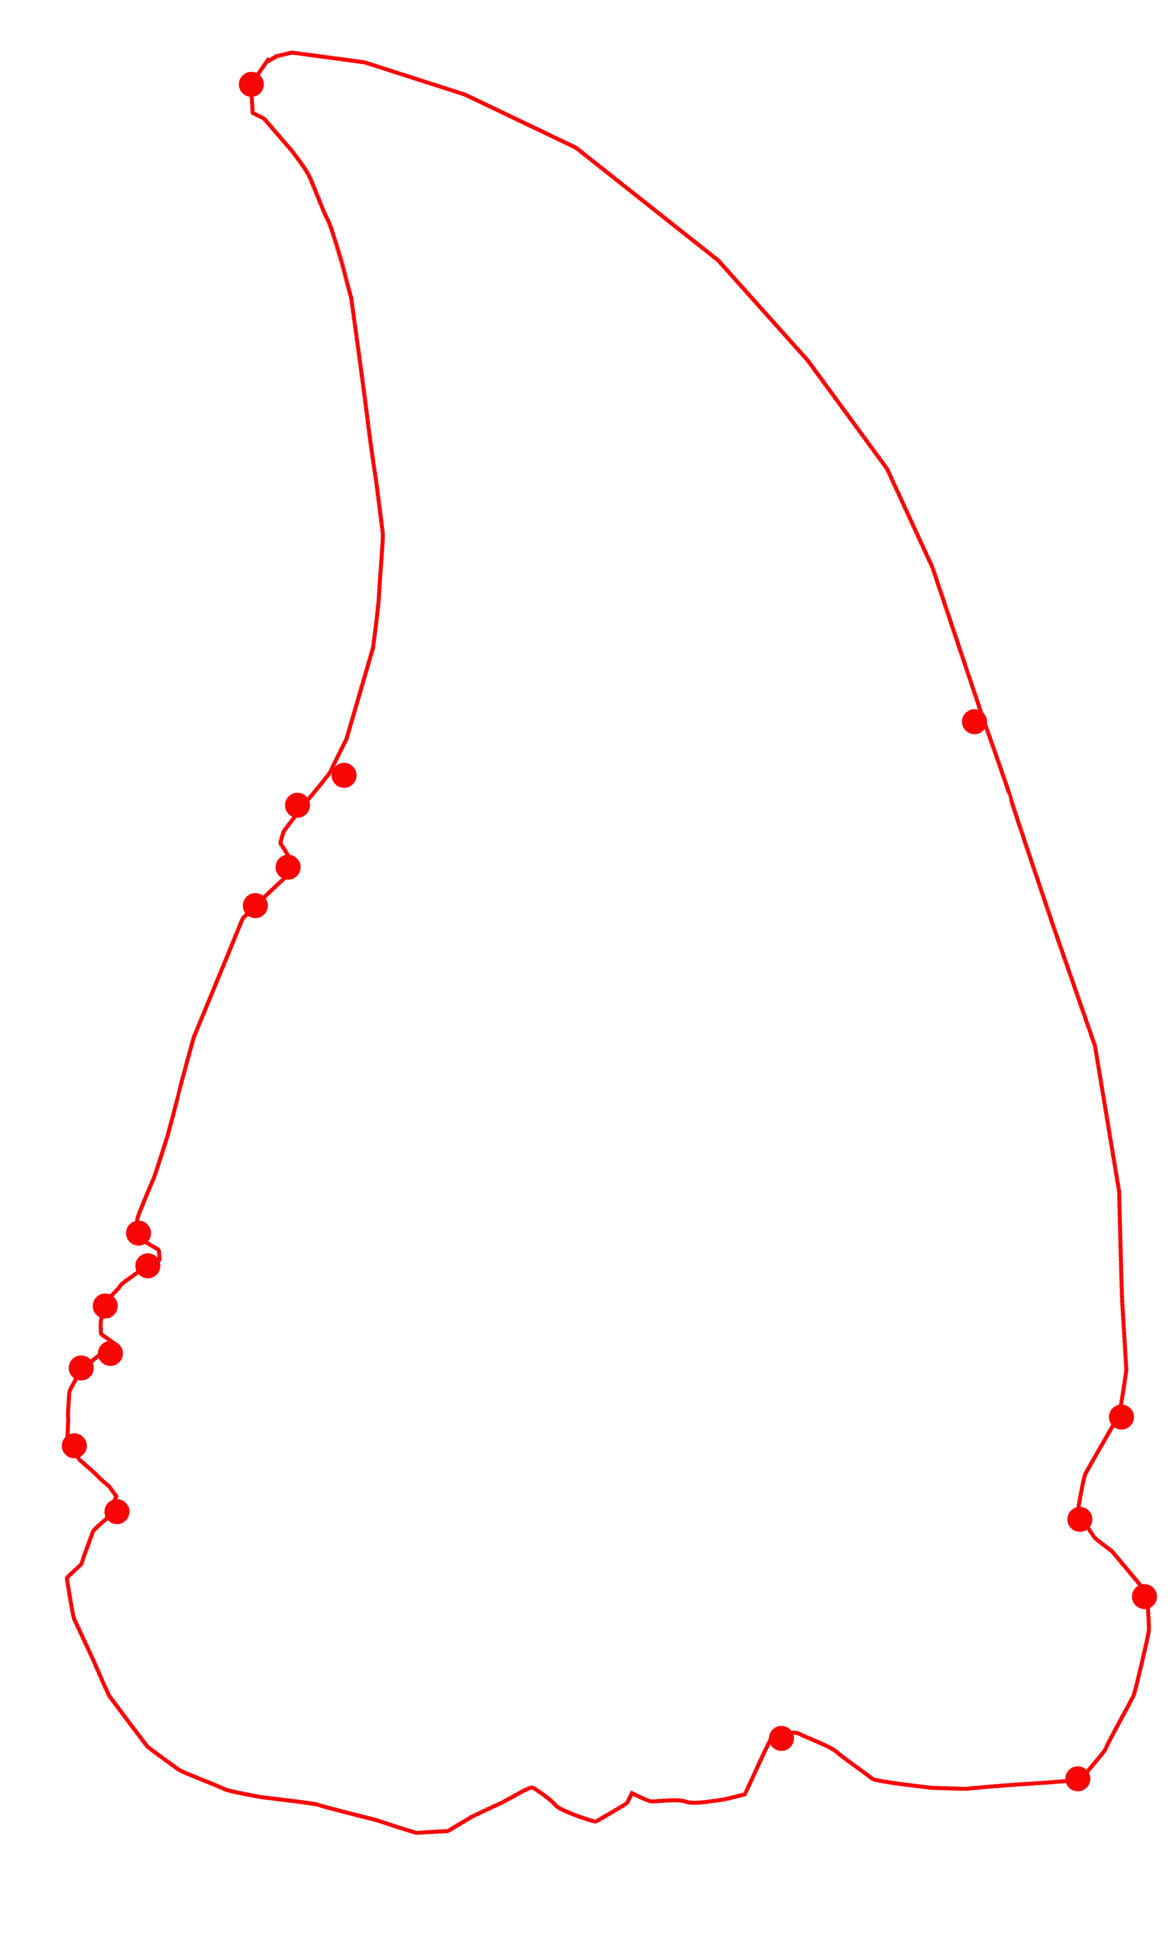
\includegraphics[scale=.3]{images/mglandmarksline}}
    \vspace{1.2cm}
  	\hspace{1.5cm}{\large{\textcolor{colorone}{\textbf{How to locate the landmarks automatically}?}}}
  	 %\begin{tikzfigure}[]
    	 % 	\centering
    	 %	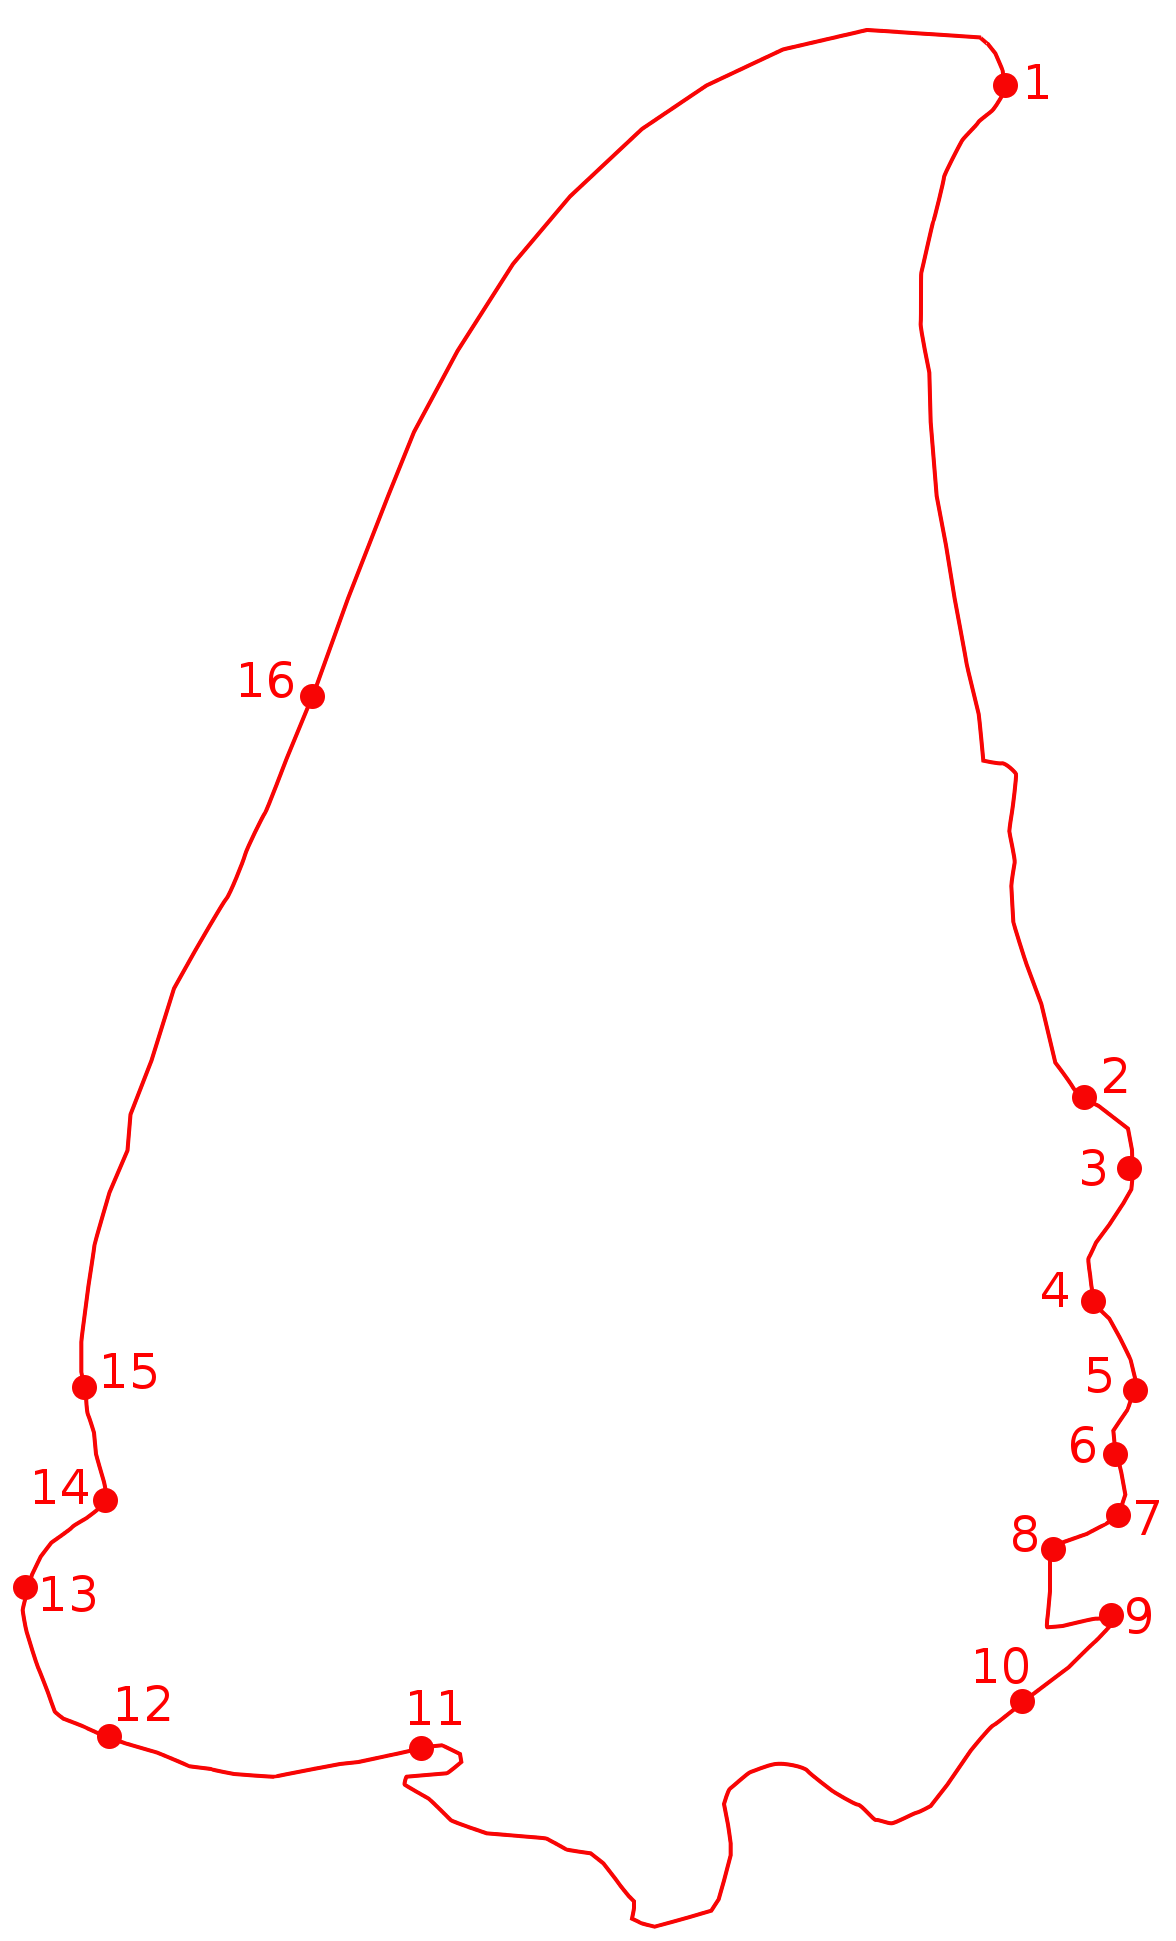
\includegraphics[scale=.28]{images/mlandmarksline}~~~~~~
    	 % 	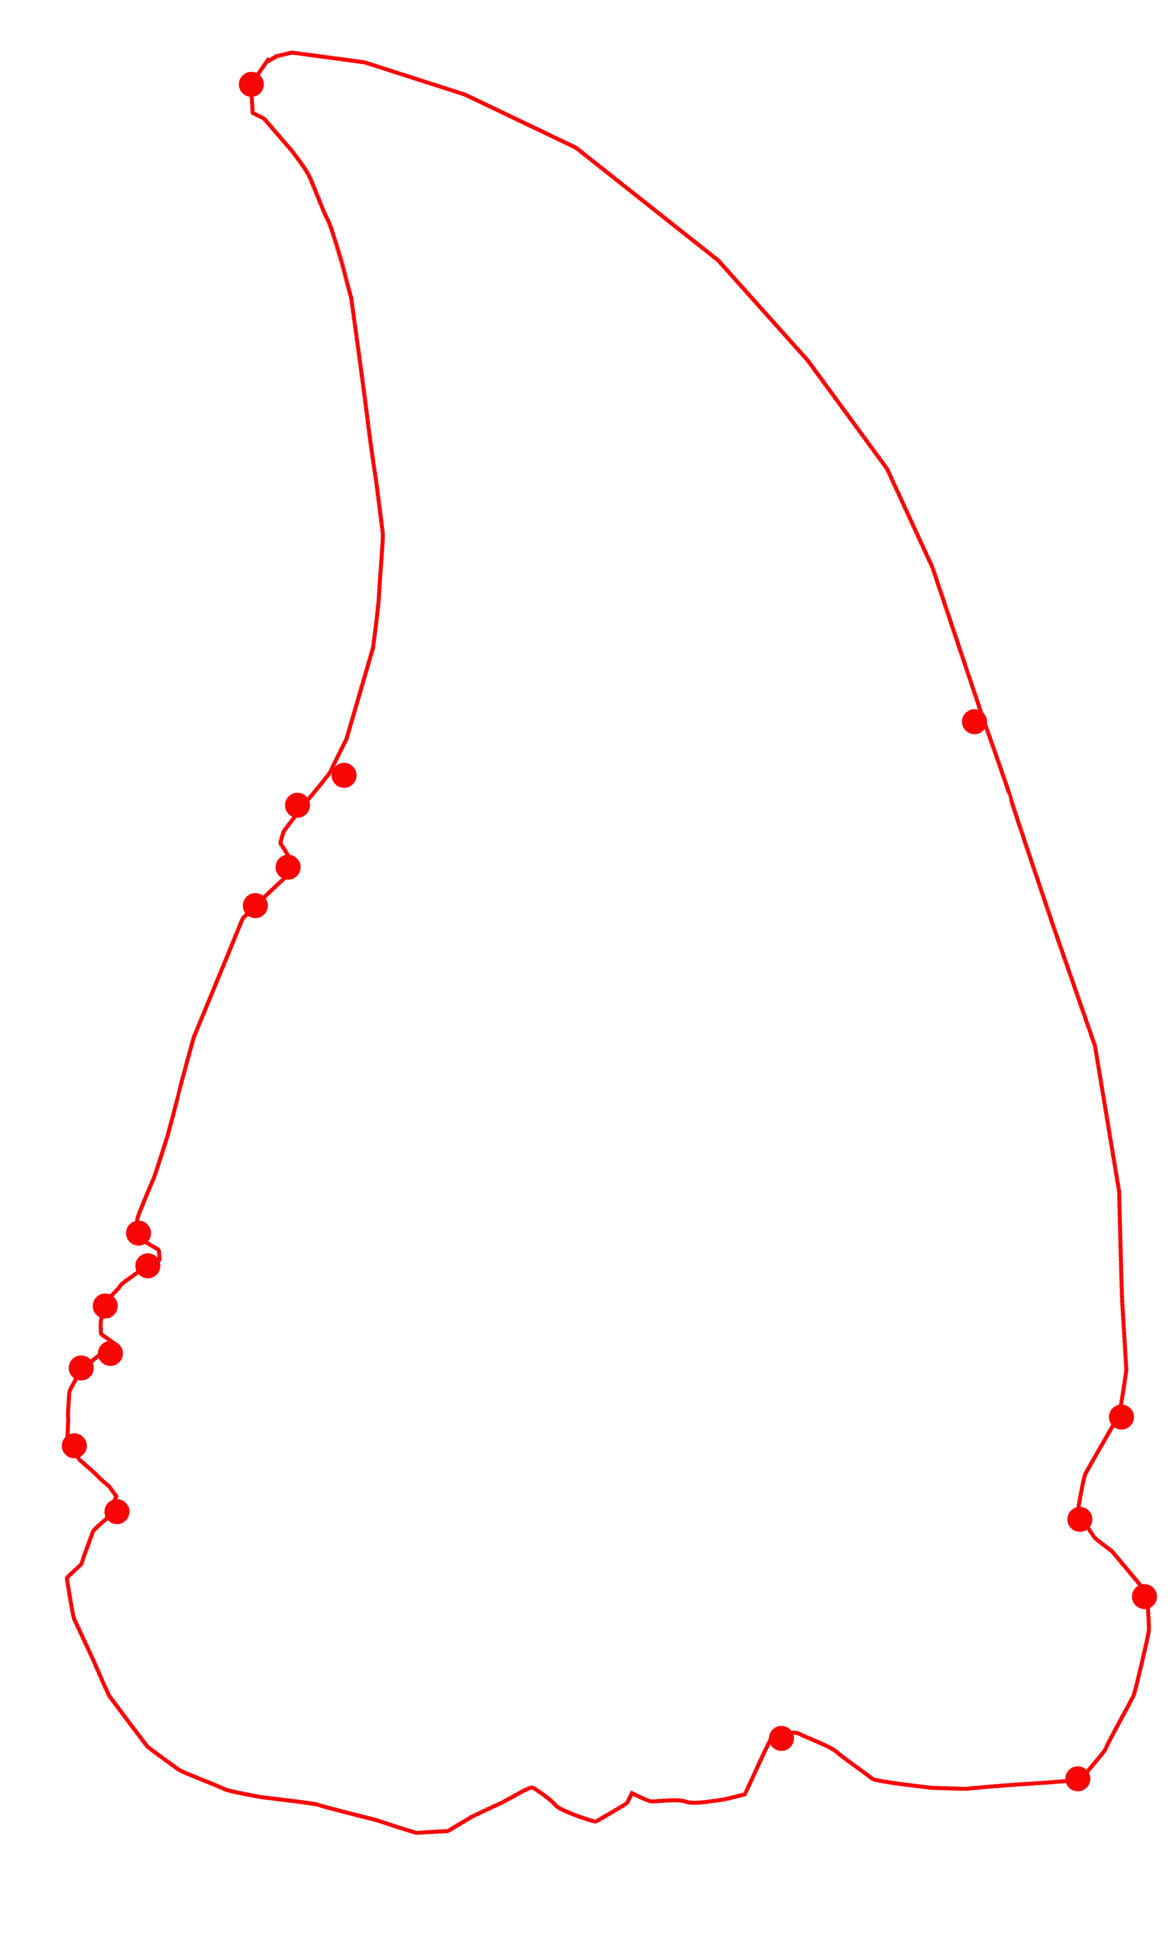
\includegraphics[scale=.28]{images/mglandmarksline}
    	 % \end{tikzfigure}
    
  }
  

  %%%%%%%%%% ------------------------------------------ %%%%%%%%%%
  \blocknode{SIFT} %
  {
  	\begin{itemize}
  		\item SIFT descriptor\cite{lowe2004distinctive} is used to extract features from images. 
  It includes four steps:
	    \begin{itemize}
    			\item Scale-space extrema detection
    			\item Keypoints localization
    			\item Orientation assigment
    			\item Keypoints descriptor
    		\end{itemize}
    		\item \textbf{\underline{Limitation:}} The obtained results from original SIFT method \\ set \textcolor{colorthree}{\textbf{many landamark candidates}}.
	    \item \textbf{\underline{Solution:}} Reducing the searching space before computing\\
    the SIFT descriptors.  
    \end{itemize} 
    \Put(25,12){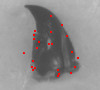
\includegraphics[scale=3.8]{images/siftc}}
  }
 
 %%%%%%%%%%%%%%%%%%%%%%%%%%%%%%%%%%%%%%%%%%%%%%%%%%%%%%%%%%%%%%%%%%%%%%%%%%
  \blocknode{Proposed method}
  {
  	\begin{itemize}
  		\item \textbf{\underline{Input:}} 
		\begin{itemize}
			\item Model image
			\item Model manual landmarks
			\item Scene image
		\end{itemize}		  		
  		\item \textbf{\underline{Output:}} 
		\begin{itemize}
			\item Landmarks of scene image
		\end{itemize}		  				
  		\item \textbf{\underline{Steps:}}
  		\begin{itemize}
  			\item Shape identification: \\ segmentation and registration
  			\item SIFT and landmarks
  		\end{itemize}
  	\end{itemize}
  	%\begin{tikzfigure}
    	%  	\centering
    	%  	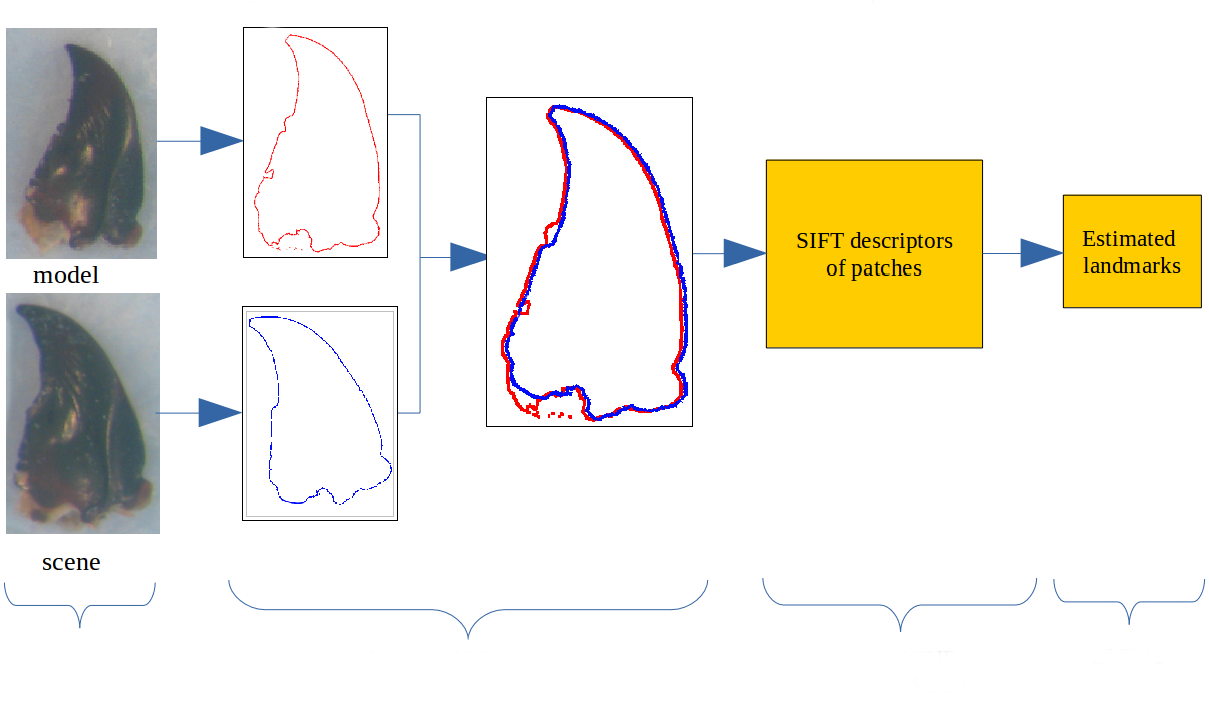
\includegraphics[scale=.5]{images/method2}
    	%  \end{tikzfigure}
    \Put(14.4,13){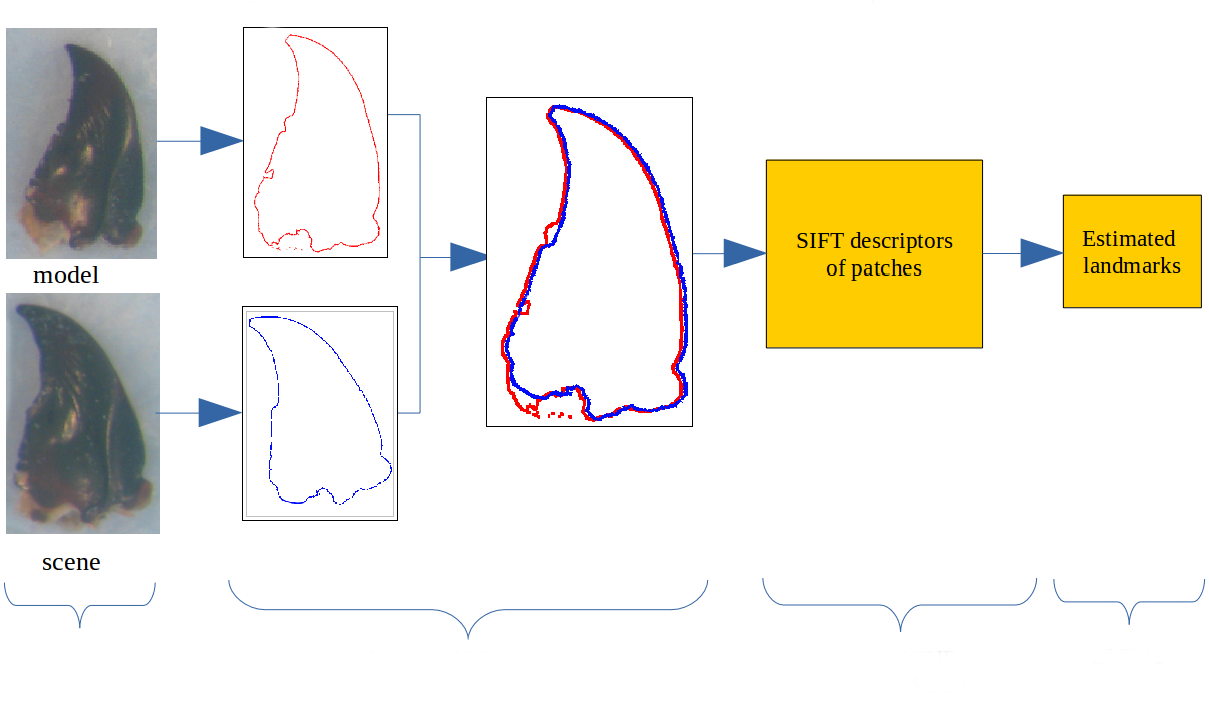
\includegraphics[scale=.5]{images/method2}}
  }
  
  
  %\useplainblocktemplate{3}
  %\plainblock[0]{($(currenty)+(2,0)$)}{35}{} %
  %{
    
  %  abc
  %  }
  \newcommand{\itemcolor}[1]{% Update list item colour
  	\renewcommand{\makelabel}[1]{\color{#1}\hfil ##1}}
 \blocknode%
  {Segmentation}%
  {
    \begin{dingautolist}{182}
    		\itemcolor{colorone}
		\item Converting the image to binary one by applying a \textcolor{colorthree}{\textbf{threshold}} determined by histogram analysis\cite{leestimating}.
		\item Contours points are extracted by Canny algorithm\cite{canny1986computational}. The thresholds ratio in Canny: $T_{lower} = (1/3) \times T_{upper}$, in which $T_{lower}$ equals to the threshold value in step 1.
    \end{dingautolist}
  }
  
  \blocknode{Registration}%
  {   Model and scene images are segmented to extract the contours points. The contours points are registered by applying \textbf{P}rincipal \textbf{C}omponent \textbf{A}nalysis\cite{jolliffe2002principal} \textbf{I}teration (PCAI).
 \begin{dingautolist}{182}
    		\itemcolor{colorone}
    		\item Compute the centroid point and principal axis of each list of contour points,
    		\item Compute the \textcolor{colorthree}{\textbf{translation}} and \textcolor{colorthree}{\textbf{rotation}} values between two lists of contour points,
    		\item \textcolor{colorthree}{\textbf{Register}} the two lists of contour points,
    		\item Sort the contour points of scene image followed y-direction,
    		\item Select a subset of contour points of scene image and repeat step 1,
    		\item PCAI stop automatically when the \textcolor{colorthree}{\textbf{angle difference}} between two 
    	lists of contour points is less than \textcolor{colorthree}{\textbf{$1.5$ degree}}.
    \end{dingautolist}
  }
  %%%%%%%%%%%%% NEW COLUMN %%%%%%%%%%%%%%% 
  \startsecondcolumn 

  %%%%%%%%%% ------------------------------------------ %%%%%%%%%%
  


  
  %%%%%%%%%% ------------------------------------------ %%%%%%%%%%
  
\blocknode{SIFT and landmarks}%
  {   
  	\begin{tikzfigure}
    	 \centering
    	 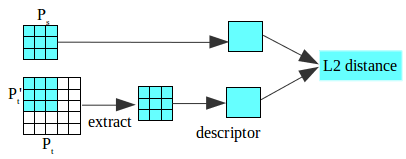
\includegraphics[width=0.7\textwidth]{images/illustration}
    \end{tikzfigure}
    \begin{dingautolist}{182}
    		\itemcolor{colorone}
    		\item A \textcolor{colorthree}{\textbf{patch}} $P_m$ is initialized at each manual landmark of model image (size of $9\times9$),
    		\item Calculating the SIFT descriptor for $P_m$,
    		\item At the same position in the scene image, a patch $P_s$ is created (size of $36\times36$),
    		\item For each pixel in $P_s$, a patch $P'_s$ is extracted with the same size than $P_m$,
    		\item Calculating the SIFT descriptor for all $P'_s$,
    		\item Computing the distance between the descriptor of $P_m$ and each $P'_m$,
    		\item At the end, the pixel that has the \textcolor{colorthree}{\textbf{minimum distance}} with $P_m$ is kept.
    \end{dingautolist}
  }

  %%%%%%%%%% ------------------------------------------ %%%%%%%%%%
  %\calloutblock{($(box.south east)-(8,-2)$)}
  %{($(box.south east)-(16,2)$)}
  %{30cm}
  %{
  % There are also callout blocks that allow for a more interesting layout of the poster. 
  %  \begin{itemize}
  %  \item[] \textbackslash calloutblock[rotate angle]\{from
  %    coordinate\}\{coordinate\}\{Block Width\}\{Block Content\} 
  %  \end{itemize}
  %  The alias for such blocks is \emph{note}.
  %}


  %% to place the next node centered vertically in the second column, we can
  %% obtain the y-coordinate of the previous node using macro
  %% \getcurrentrow{note}, where note is the alias of the callout node, and
  %% then specify the coordinate of the next node using coordinate (currentrow)
  %\getcurrentrow{note}


  %% a plain block
  %% #1 - rotate angle (optional), #2 - where, #3 - width, #4 - title, #5 - text
  %%%%%%%%%% ------------------------------------------ %%%%%%%%%%
  %\plainblock{($(currentrow)+(xshift)-(yshift)$)}%[($(currenty)+(0,10)$)]%
  %{32}{Plain blocks} %
  %{These blocks are similar to callout blocks. They allow for specifying the
  %  title of the block.
  %  \begin{itemize}
  %  \item[] \textbackslash plainblock[rotate angle]\{coordinate\}\{Block Width\}\{Block
   %   Title\}\{Block Content\} 
   % \end{itemize}
  %}


 
  %% the coordinate (currenty) is used in the default placing of the next blocknode
 %\getcurrentrow{note}
 %\coordinate (currenty) at ($(currentrow)+(xshift)-(yshift)$);



   %%%%%%%%%%%%% NEW COLUMN %%%%%%%%%%%%%%% 
  %% (if column number is 3)
 % \startthirdcolumn

  %%%%%%%%%% ------------------------------------------ %%%%%%%%%%
  \blocknode {Results on right mandibles}
  {
  	\begin{itemize}
  		\item Highest accuracy: $1^{st}$ landmark with \textcolor{colorthree}{\textbf{$98.62\%$}}
  		\item Lowest accuracy: $13^{th}, 14^{th}$ landmark with app. $75\%$
  	\end{itemize}
  	\Put(21.5,-21){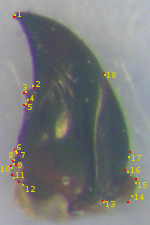
\includegraphics[scale=1.8]{images/md_rs}}
  	\Put(2,-21.5){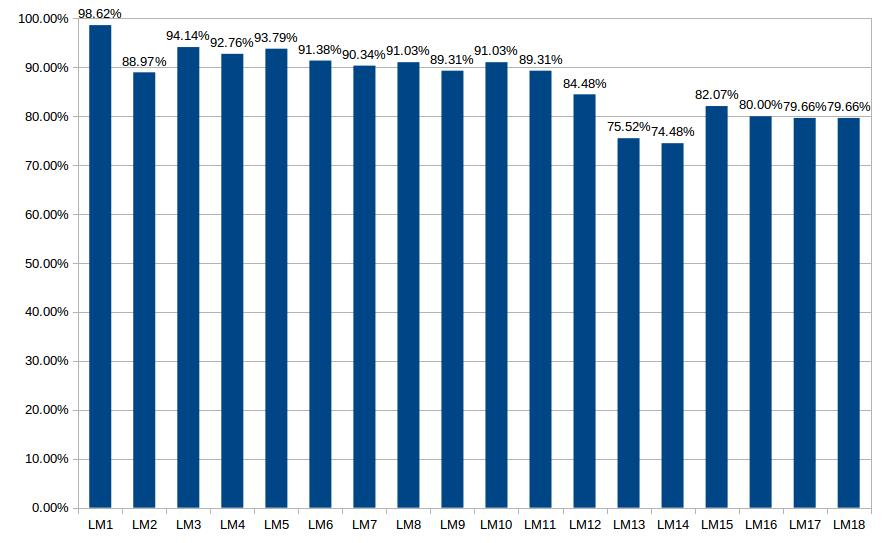
\includegraphics[scale=.6]{images/md_chartlms}}
  	\vspace{10cm}
  	%\begin{tikzfigure}[]
    	%	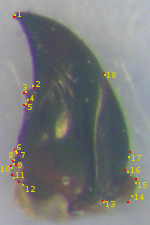
\includegraphics[scale=1.7]{images/md_rs}~~
    	%	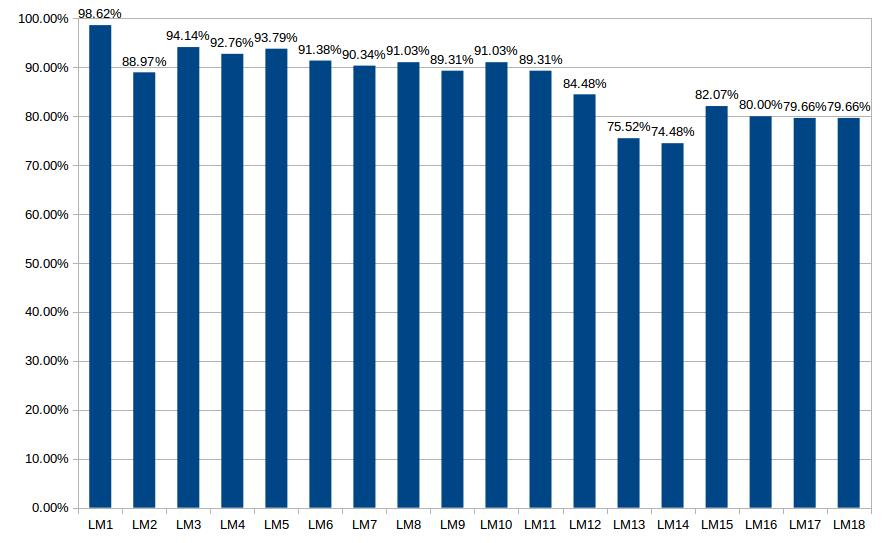
\includegraphics[scale=.6, left]{images/md_chartlms}
    %\end{tikzfigure}
  }

\blocknode {Results on left mandibles}
  {
  \begin{itemize}
  		\item Highest accuracy: $1^{st}$ landmark with \textcolor{colorthree}{\textbf{$93.01\%$}}
  		\item Lowest accuracy: $11^{th}, 12^{th}$ and $16^{th}$ landmark \\ from  $60\%$ to app. $63\%$
  	\end{itemize}
  	\Put(22,-22){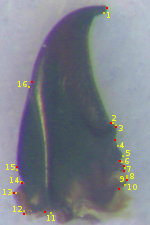
\includegraphics[scale=1.8]{images/mg_rs}}
  	\Put(3,-22.5){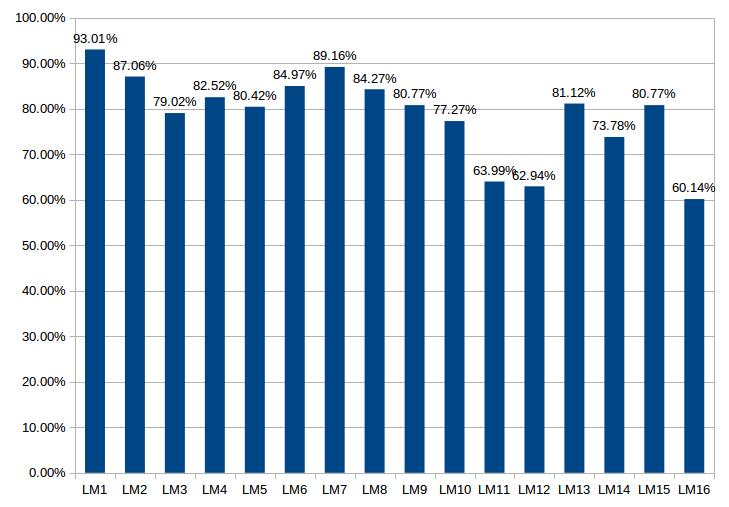
\includegraphics[scale=0.7]{images/mg_chartlms}}
  	\vspace{10.7cm}
  	%\begin{tikzfigure}[]
    	%\centering
    	%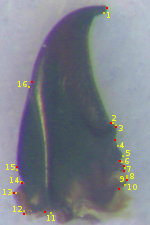
\includegraphics[scale=1.7]{images/mg_rs}~~
    	%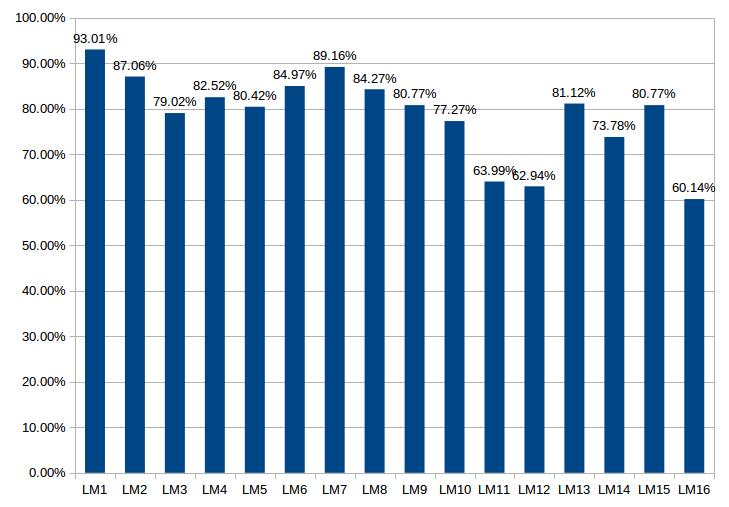
\includegraphics[scale=.785, left]{images/mg_chartlms}
    %\end{tikzfigure}
  }
%%%%%%%%%% ------------------------------------------ %%%%%%%%%%
\blocknode{Conclusions}
{
	\begin{itemize}
		\item A solution based on SIFT descriptor for landmark estimation is presented,
		\item The results show that method \textcolor{colorthree}{\textbf{succeed in locating}} all landmarks in  request images,
		\item The accuracy of method is sufficient to be \textcolor{colorthree}{\textbf{proposed to biologists}} as a \textcolor{colorthree}{\textbf{replacement of manual positioning}}, and to characterize the shape.
	\end{itemize}
}

%%%%%%%%%% ------------------------------------------ %%%%%%%%%%
  \blocknode%
  {Bibliography}%
  {
  \renewcommand{\refname}{\vskip -3.45cm}
   \bibliographystyle{abbrv}
%   \renewcommand{\bibname}{}
	\bibliography{../references}
  }


\end{tikzpicture}


\end{document}




